
We construct the index structure on features. Our index structure is a chain hashing structure. For a give data point to be inserted in to the structure, for each of it features, we hash the feature and insert the reference to the data point in the chain. The motivation behind the use of an inverted index structure comes from the use of the tf-idf (term frequency-inverse document frequency) in text mining and information retrieval. Also chemical data is known to have an almost power law distribution for the presence of features in the data points and we wish to exploit this.

\section{Point Query}

Point query operation can be very effectively 
implemented in the inverted index structure. To perform this operation we maintain a list of candidate nodes, which needs to be explored sequentially. Our aim is to prune the candidate list as much as possible. This pruning is done by the following observation.\\
Given a point $p$ we look at all its features, and find the list of all nodes associated with the features. It is a straight forward observation that $p$ is present in the data-set only if, it is in the intersection of all the associated point list. This reduces our candidate list to a size, atleast as small as the smallest list, among all the features present in $p$ .\\

\section{Range Query and K-nn}
Range query and K-nn are much more complicated queries, when compared to a point query. The candidate set in this case is much more diverse and distributed. For example the candidate set for a Range query will be the union of all the point lists associated with the features of $p$, which is the worst case is of the order of $N$. We try to prune this by observing that the minimum number of features in a point is 7, hence we can remove the top 6 features from the index with out affecting the accuracy of searching. But this pruning does not result in any improvement in performance. We shall discuss this further the sections below.\\

\section{Baseline technique for Range Search}
\label{sec:base}
 Given a query q, which has features $f_1, f_2,...f_{N_q}$ we take a union of all compounds present in atleast one of these features and then proceed with a linear search. This is described in detail below.

\begin{enumerate}
	\item We keep a hash table where every feature has a pointer to the set of points which contains that feature itself.
	\item Let the feature $f_1$ of query q be present in the points $p_1,p_2,...p_M$. Let this set be $S_1$.
	\item We take a union of all such sets $S_1, S_2,...S_{N_q}$ defined as the set $S_q$
	\item We do a linear search on the compounds present in this set.
	\item The answer are the subset of points of the set $S_q$ which fall within threshold t of the query.	 
\end{enumerate}


\begin{figure}[ht]	
\centering
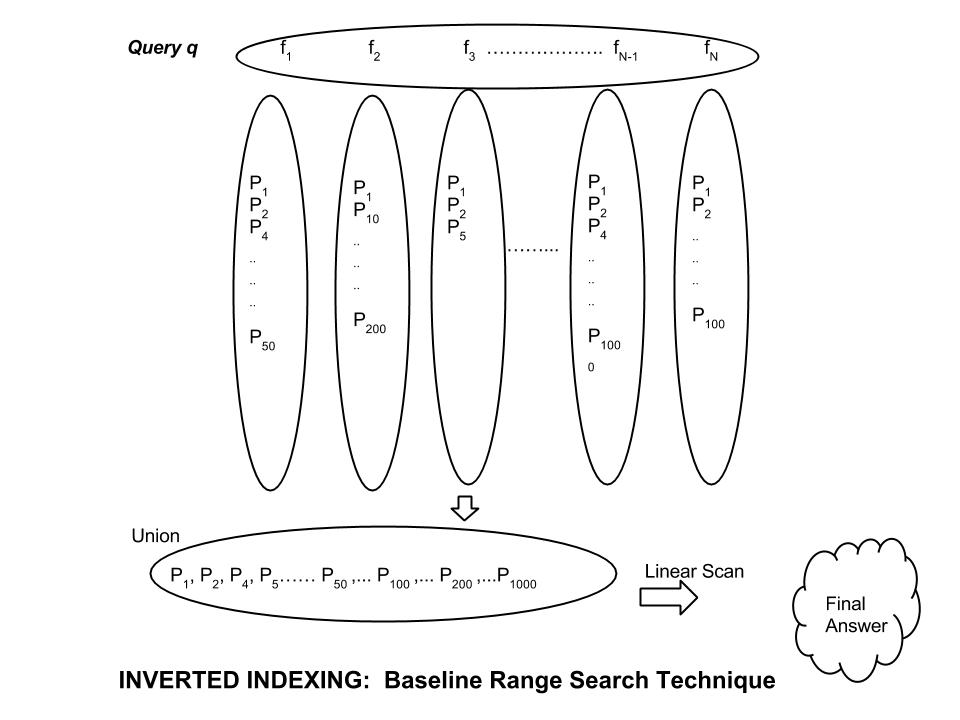
\includegraphics[width=1 \columnwidth]{img/image0c.jpg}
\caption{Inverted Indexing: Procedure Diagram}
\label{fig: invert}
\end{figure}




\section{A Pruning bound for binary fingerprints}
\label{sec:prune1}
We state theorems in this section which will derive the bounds we utilize in our proposed range search technique described in the \autoref{sec:prune1.1}. The technique will build on the baseline algorithm mentioned in \autoref{sec:base}.

Pruning of a feature can be described as cutting out all the points containing  particular the feature from the candidate result set of a range search query process. Pruning out a feature containing many number of points will help save on the computation time spent on similarity calculation of the database compounds with the query compound.


\begin{thm}
\label{thm1bound}
For a case of binary fingerprints, given a query $q$ and a threshold $t$, consider the feature $f_i$. If $P$ is the set of points from the database which has the feature $f_i$ set to 1, then we can prune all such points $p_j$ of P from being present in the candidate range search query result set for query compound $q$ if the point $p_j$ has only $f_i$ in common with the query $q$ and it follows the following bound. 

\begin{equation}
\label{eq:boun}
\frac{1}{N_q - 1 + V_{i}}  < 1-t
\end{equation}

where $N_q$ is the number of features in query q and $V_{i}$ is the minimum number of features present among all points having the feature $f_i$

\end{thm}


\begin{proof}
\label{proof1}
Our assumption is that a point $p_j$ from P is such that it has only $f_i$ in common with the query $q$  
 
The maximum Tanimoto similarity $S_{max}(p_j,q)$ such a point $p_j$ can have with the query point $q$ is given by
\begin{equation}
\label{eq:max}
S_{max}(p_j,q)=\frac{1}{N_q - 1 + V_{1}}
\end{equation}

This is because the Tanimoto similarity as described in \autoref{eq:tan} is such that the numerator equals the number of common features which according to the assumption is 1. The denominator in the above equation is the minimum size of the union of the feature set of any such point $p_j$ from $P$ and the query point $q$.
The equation gives us the right hand side of the bound 
in \autoref{eq:boun}. 

The minimum similarity $S_{min}$ required with the query for a candidate compound to be in the result of the range search is 1-$t$ where t is the maximum distance threshold.

If the following equation were to hold:
\begin{equation}
\label{eq:min}
	S_{max}(p_j,q) < S_{min}
\end{equation}
Then maximum possible similarity of a point would be less than the minimum required similarity for the point to be considered a candidate, hence we could prune the set of all such points and save time from doing its similarity computation with the query. 

From \autoref{eq:boun},\autoref{eq:max} and \autoref{eq:min}, we get the following bound,
\begin{equation}
\frac{1}{N_q - 1 + V_{i}}  < 1-t
\end{equation}

which is as the theorem states.

\end{proof}


Now let us consider pruning of multiple features together. 


\begin{thm}
\label{thm2bound}
For a case of binary fingerprints, given a query $q$ and a threshold $t$, consider the feature set $F=f_1, f_2,...f_M$. If $P$ is the set of points from the database which has atleast one of the features$f_k$  $(f_k~\in F)$, set to 1 then we can prune all such points $p_j$ of P from being present in the candidate range search query result set for query compound $q$ if the point $p_j$ does not have any other common feature other than in the set $F$, and it follows the following bound. 

\begin{equation}
\label{eq:boun2}
\frac{M}{N_q - 1 + \min\limits_{i\in~(1,M)}(V_i) } < 1-t 
\end{equation}

where $M$ is the number of features in the set $F$,$N_q$ is the number of features in query q and $V_{i}$ is the minimum number of features present among all points having the feature $f_i$.




\end{thm}

\begin{proof}
\label{proof2}
The proof is similar to how Theorem \autoref{thm1bound} is derived. 

%%%%%%%%%%%%%


Our assumption is that a point $p_j$ from P is such that it can have only a feature from the set $F=f_1, f_2,...f_M$ in common with the query $q$  
 
The maximum Tanimoto similarity $S_{max}(p_j,q)$ such a point $p_j$ can have with the query point $q$ is given by
\begin{equation}
\label{eq:max2}
S_{max}(p_j,q)=\frac{M}{N_q - 1 + \min\limits_{i\in~(1,M)}(V_i) } < 1-t 
\end{equation}

According to our assumption, the maximum possible value for the numerator in the score for Tanimoto similarity as described in \autoref{eq:tan} is $M$ when all features from the set are common to the query and the point $p_j$. The denominator in the above equation gives the minimum size of the union of the feature set of any such point $p_j$ from $P$ and the query point $q$. 
The rest of the proof is similar to how it is explained in the proof of Theorem \autoref{thm1bound}.
\end{proof}


\section{Improvised Range Search technique}
\label{sec:prune1.1}
We can now present a modified algorithm for a range search using pruning of the features. For a case of binary fingerprints, given a query $q$ and a threshold  $t$, the indexing algorithm goes as follows (As used earlier, $N_q$ is the number of features in query q and $V_{i}$ is the minimum number of features present among all points having the feature $f_i$.)

\begin{enumerate}
	\item We sort the features of the query q, $f_1,f_2,...f_{N_q}$ in descending order of popularity i.e. the feature present in most of the points is at the start.
	
	\item Consider feature $f_1$. Let's say we want to prune this feature. We are concerned with points having this feature but not having any of the other features of the query point. 
	
	\item Hence if  distance threshold is t and the following holds (as described in \autoref{eq:boun}) 
	\begin{equation}
	\frac{1}{N_q - 1 + V_{1}}  < 1-t
	\end{equation}
	
we can prune the feature $f_1$		
	
	\item We continue a greedy approach, where we consider the next feature $f_2$ and try to prune both the features $f_1$ and $f_2$ together.
	
	\item Hence if till the $i^{th}$ feature is considered, if j features (call it set $R$) have been pruned till now, we can prune the $i^{th}$ feature as well if the following holds (as described in \autoref{eq:boun2})
	\begin{equation}
	\label{eq: greedy}
	\frac{j+1}{N_q - 1 + min(V_{i}, \rho)} < 1-t 
	\end{equation}
	
where 	$\rho$ is the minimum  number of features present in any point containing atleast one of the features pruned until now i.e $\rho = \min\limits_{k\in R} V_k$

	\item This process is continued till we reach the end of the sorted feature list.
	
	\item We now follow the baseline range search technique described in \autoref{sec:base} but on the set of features of the query compound not pruned till now. 
	
\end{enumerate}

The main idea behind the use of the greedy algorithm is to prune as many as points as possible. Hence the sorting of the features in order of their popularity. We also tried sorting based on other scores but none gave as good as the results obtained by using popularity for sorting. 

Consider the pruning process. If say we prune $f_l$ we need to consider features until $f_{l-1}$ which we have pruned till now. Lets say there is a point $p_o$ which also has a feature not seen till now , say $f_{l+q}, q\in(1,M-l)$ . We do not care about such points since they would be considered in the candidate set for out range search query if in the future $f_{l+q}$ is not pruned. We only care for those points which would not be present in any further features beyond feature $f_l$. 

\section{Extension to non-binary fingerprints}	
\label{sec:prune2}

We can extend Theorem 3 and Theorem 4 to non-binary fingerprints as follows:

%%%%


\begin{thm}
\label{thm3bound}
For the case of non-binary fingerprints, given a query $q$ and a threshold $t$, consider the feature $f_i$. If $P$ is the set of points from the database which has non-zero $f_i$ value, then we can prune all such points $p_j$ of P from being present in the candidate range search query result set for query compound $q$ if the point $p_j$ has only $f_i$ in common with the query $q$ and it follows the following bound. 

\begin{equation}
\label{eq:boun3}
\frac{min(j_i,W_i)}{S_q - W_i -k_i+ l_i + max (k_i, V_i)}  < 1-t
\end{equation}
Here $j_i$ is the maximum feature value taken for the feature $f_i$, $W_i$ is the first feature value of query $q$, $S_q$ is the sum magnitude of the feature values of the query $q$, $k_i$ is the is the minimum feature value taken for the feature $f_i$, $l_i$ is the minimum sum of feature values for any point containing the feature $f_i$ and $t$ is the threshold similarity


\end{thm}


\begin{proof}
\label{proof3}

This follows from the definition of the similarity measure for non-binary fingerprints as described in \autoref{eq:minmax}. If the two compounds in question, $q$  and $p_j$ have only one feature $f_i$ in common, then accordingly the maximum numerator value for the similarity score would be $min(j_i,W_i)$ while the denominator would take a minimum value of $S_q - W_i -k_i+ l_i + max (k_i, V_i)$. The rest of the proof follows as in proof of Theorem \autoref{thm1bound}.

\end{proof}



%%%%%%%%
\begin{thm}
\label{thm4bound}
For the case of non-binary fingerprints, given a query $q$ and a threshold $t$, consider the feature set $F=f_1, f_2,...f_M$. If $P$ is the set of points from the database which has atleast one non-zero $f_k$ value $(f_k~\in F)$, then we can prune all such points $p_j$ of P from being present in the candidate range search query result set for query compound $q$ if the point $p_j$ does not have any other common feature other than in the set $F$, and it follows the following bound. 
\begin{equation}
\label{eq:boun4}
\frac{\sum\limits_{i \in J}min(j_i,W_i)}{S_q - \sum\limits_{i \in J}W_i -\sum\limits_{i \in J}k_i + max_{i \in J}l_i + \sum\limits_{i \in J}max (k_i, V_i)}  < 1-t
\end{equation}	

Here $J$ is the set of features already pruned,$j_i$ is the maximum feature value taken for the feature $f_i$, $W_i$ is the $i^th$ feature value of query $q$, $S_q$ is the sum magnitude of the feature values of the query $q$ as mentioned earlier, $k_i$ is the is the minimum feature value taken for the feature $f_i$ , $l_i$ is the minimum sum of feature values for any point containing the feature $f_i$ and $t$ is the threshold similarity

\end{thm}

\begin{proof}
\label{proof4}
The proof follows from \autoref{eq:minmax} and proof of Theorem \autoref{thm2bound} \\ 
\end{proof}





%%%%%%%






%%%%%


The algorithm in \autoref{sec:prune1.1} is to be modified as follows; for step 3 of the algorithm, while considering non-binary fingerprints we have to use the following inequality to determine if feature $f_1$ can be pruned.

\begin{equation}
\label{nonbineq1}
\frac{min(j_1,W_1)}{S_q - W_1 -k_1 + l_1 + max (k_1, V_1)}  < 1-t
\end{equation}

Similarly for step 5 of the algorithm in \autoref{sec:prune1.1}: if till the $i^{th}$ feature is considered, if j features have been pruned, we can prune the $i^{th}$ feature as well if the following holds:
		
\begin{equation}
\label{nonbineq2}
\frac{\sum\limits_{i \in J}min(j_i,W_i)}{S_q - \sum\limits_{i \in J}W_i -\sum\limits_{i \in J}k_i + max_{i \in J}l_i + \sum\limits_{i \in J}max (k_i, V_i)}  < 1-t
\end{equation}	

Remaining steps remain the same.

\section{Using the Minimum Similarity Bound}

Just like in the M-tree, similar to using the triangle inequality bounds, instead of using the maximum possible similarity, we used the minimum possible similarity and use it to include all points contained by a feature.

Hence for a feature $f_1$ of a binary fingerprint query $q$, we can include all points having feature $f_1$ in our result set if the following inequality holds
\begin{equation}
\frac{1}{N_q - 1 + U_{1}}  > 1-t
\end{equation}

Here $N_q$ is the number of features in query q and $U_{1}$ is the maximum number of features present among all points having the feature $f_1$. This holds true because the right hand side of the bound represents the least possible similarity between the query and any compound having feature $f_1$. If the left hand side is greater than the similarity threshold s ($s=1-t$), than we need not undergo the min-max similarity calculation for all the chemical fingerprints.

This is a very loose lower bound and hence we observed in our results that we were unable to exploit this bound for speeding up our process.
	


\section{Splitting Features}

Another technique we considered for the binary data-set is the splitting of the heavy hitting features into two sets so that we can prune atleast the bigger set. If the bound for pruning the feature fails, then we try to split the feature into two sets so that the minimum number of features for any point in one of the sets increases and then giving a chance of the set being pruned. For this we have to sort the points in the feature in ascending order of the number of features present in the point .This procedure is applied only for the heavy hitting features since they appear in a large number of points. If we were to apply this to other features, the time spent partitioning would exceed the probable time spent in comparing all points in the partition to the query. Hence we would like to apply this only to features which are present in more than a threshold number of points.\\

\begin{figure}[ht]	
\centering
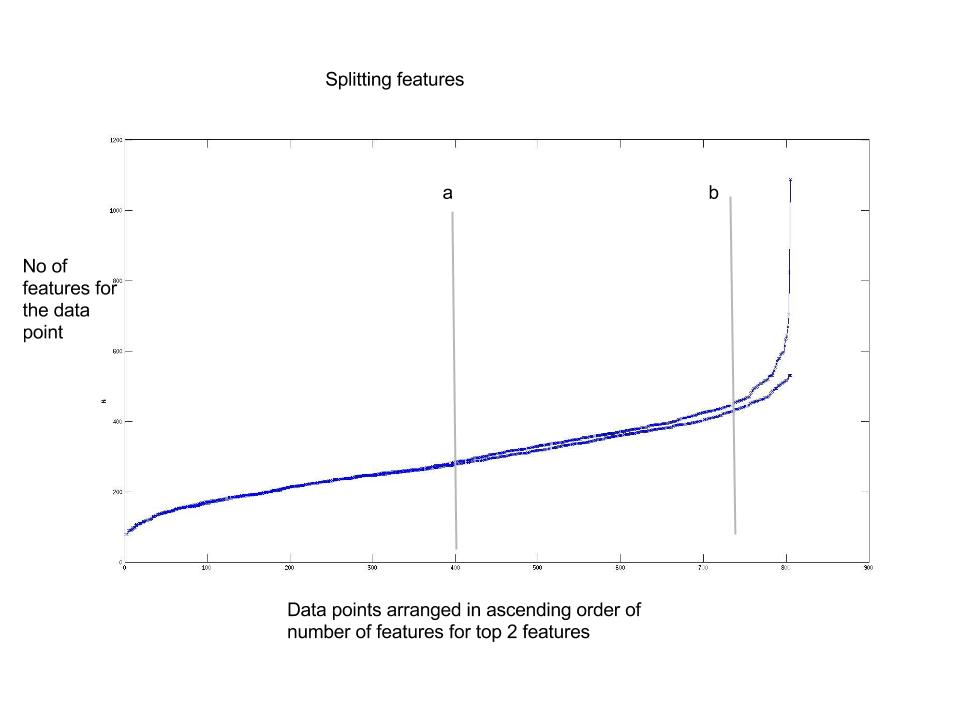
\includegraphics[width=1 \columnwidth]{img/feat_split.jpg}
\caption{Inverted Indexing: Splitting the heavy hitting features}
\label{fig:split}
\end{figure}

\autoref{fig:split} shows the number of features versus every point present for two heavy hitting features. It can be observed that the curve is almost linear, hence intuitively we wouldn't get a very large increase in the minimum number of features for the larger set of points.In \autoref{fig:split}, we can observe two lines \textit{a} and \textit{b}. If we were to split at \textit{a}(into approximately two equal sets) after sorting, our pruning bound would have a lower chance of getting  satisfied while if we were to cut at \textit{b} d(at about 90\% to 10\%) we would have a better chance of pruning the set containing the top 10 percent of the points. We were unable to get desirable results with the splitting the features method.